% !TEX encoding = UTF-8
% !TEX TS-program = pdflatex
% !TEX root = ../tesi.tex

%**************************************************************
\chapter{Introduzione}
\label{cap:introduzione}
%**************************************************************

%Introduzione al contesto applicativo.\\
%
%\noindent Esempio di utilizzo di un termine nel glossario \\
%\gls{api}. \\
%
%\noindent Esempio di citazione in linea \\
%\cite{site:agile-manifesto}. \\
%
%\noindent Esempio di citazione nel pie' di pagina \\
%citazione\footcite{womak:lean-thinking} \\

%**************************************************************

\section{Concetti chiave}
\subsection{Processi di business e process mining}
"Il \textbf{processo aziendale} (o business process) è un insieme di attività interrelate, svolte all'interno dell'azienda nell'ambito della gestione operativa delle sue funzioni aziendali, che creano valore trasformando delle risorse (input del processo) in un prodotto finale (output del processo) a valore aggiunto, destinato ad un soggetto interno o esterno all'azienda (cliente)" \cite{site:wiki-business-process}.
\\ 
Un processo è quindi caratterizzato da una sequenza di passi (attività) con lo scopo di raggiungere un obiettivo. \'E importante notare come le varie sequenze sono spesso standardizzate, di conseguenza di avranno, per la maggior parte, esecuzioni simili.
\\ 
A loro volta i processi di business sono la fonte di informazione per il process mining. 
\\
"Il \textbf{process mining} è una tecnica di process management, che permette l'analisi dei processi di business basati sui log degli eventi." \cite{site:wiki-process-mining}
\\
Il process mining quindi offre varie tecniche per estrarre informazioni utili dai log degli eventi. 
\subsubsection{Log degli eventi}
In generale un sistema informativo (che può essere un database o un ERP) genera dati realtivi agli eventi avvenuti in forma di log, tipicamente per registrare e tracciare i cambiamenti avvenuti allo stato del sistema.
Spesso questi dati sono organizzati in forma tabulare e prendono la forma di un log di eventi.
Un log di eventi (o \textit{event log}) quindi, è una collezione di dati relativi ad eventi registrata e tracciata da un sistema informativo e conservata in file strutturati (es. CSV, XES, ecc.).
Si parla di \textbf{traccia} quando ci si riferisce ad un insieme di eventi con lo stesso case id, quindi un event log può essere visto anche come una collezione di tracce.

Rappresenta l'impronta digitale elettronica delle varie operazioni aziendali. 
Va osservato che, in generale, un log non è mai direttamente utilizzabile, può infatti contenere gap, inconsistenze e ripetizioni. Si ritiene quindi necessario delle operazioni di preparazione, che permettono di filtrare e pulire i dati.

\begin{figure}[H] 
    \centering 
    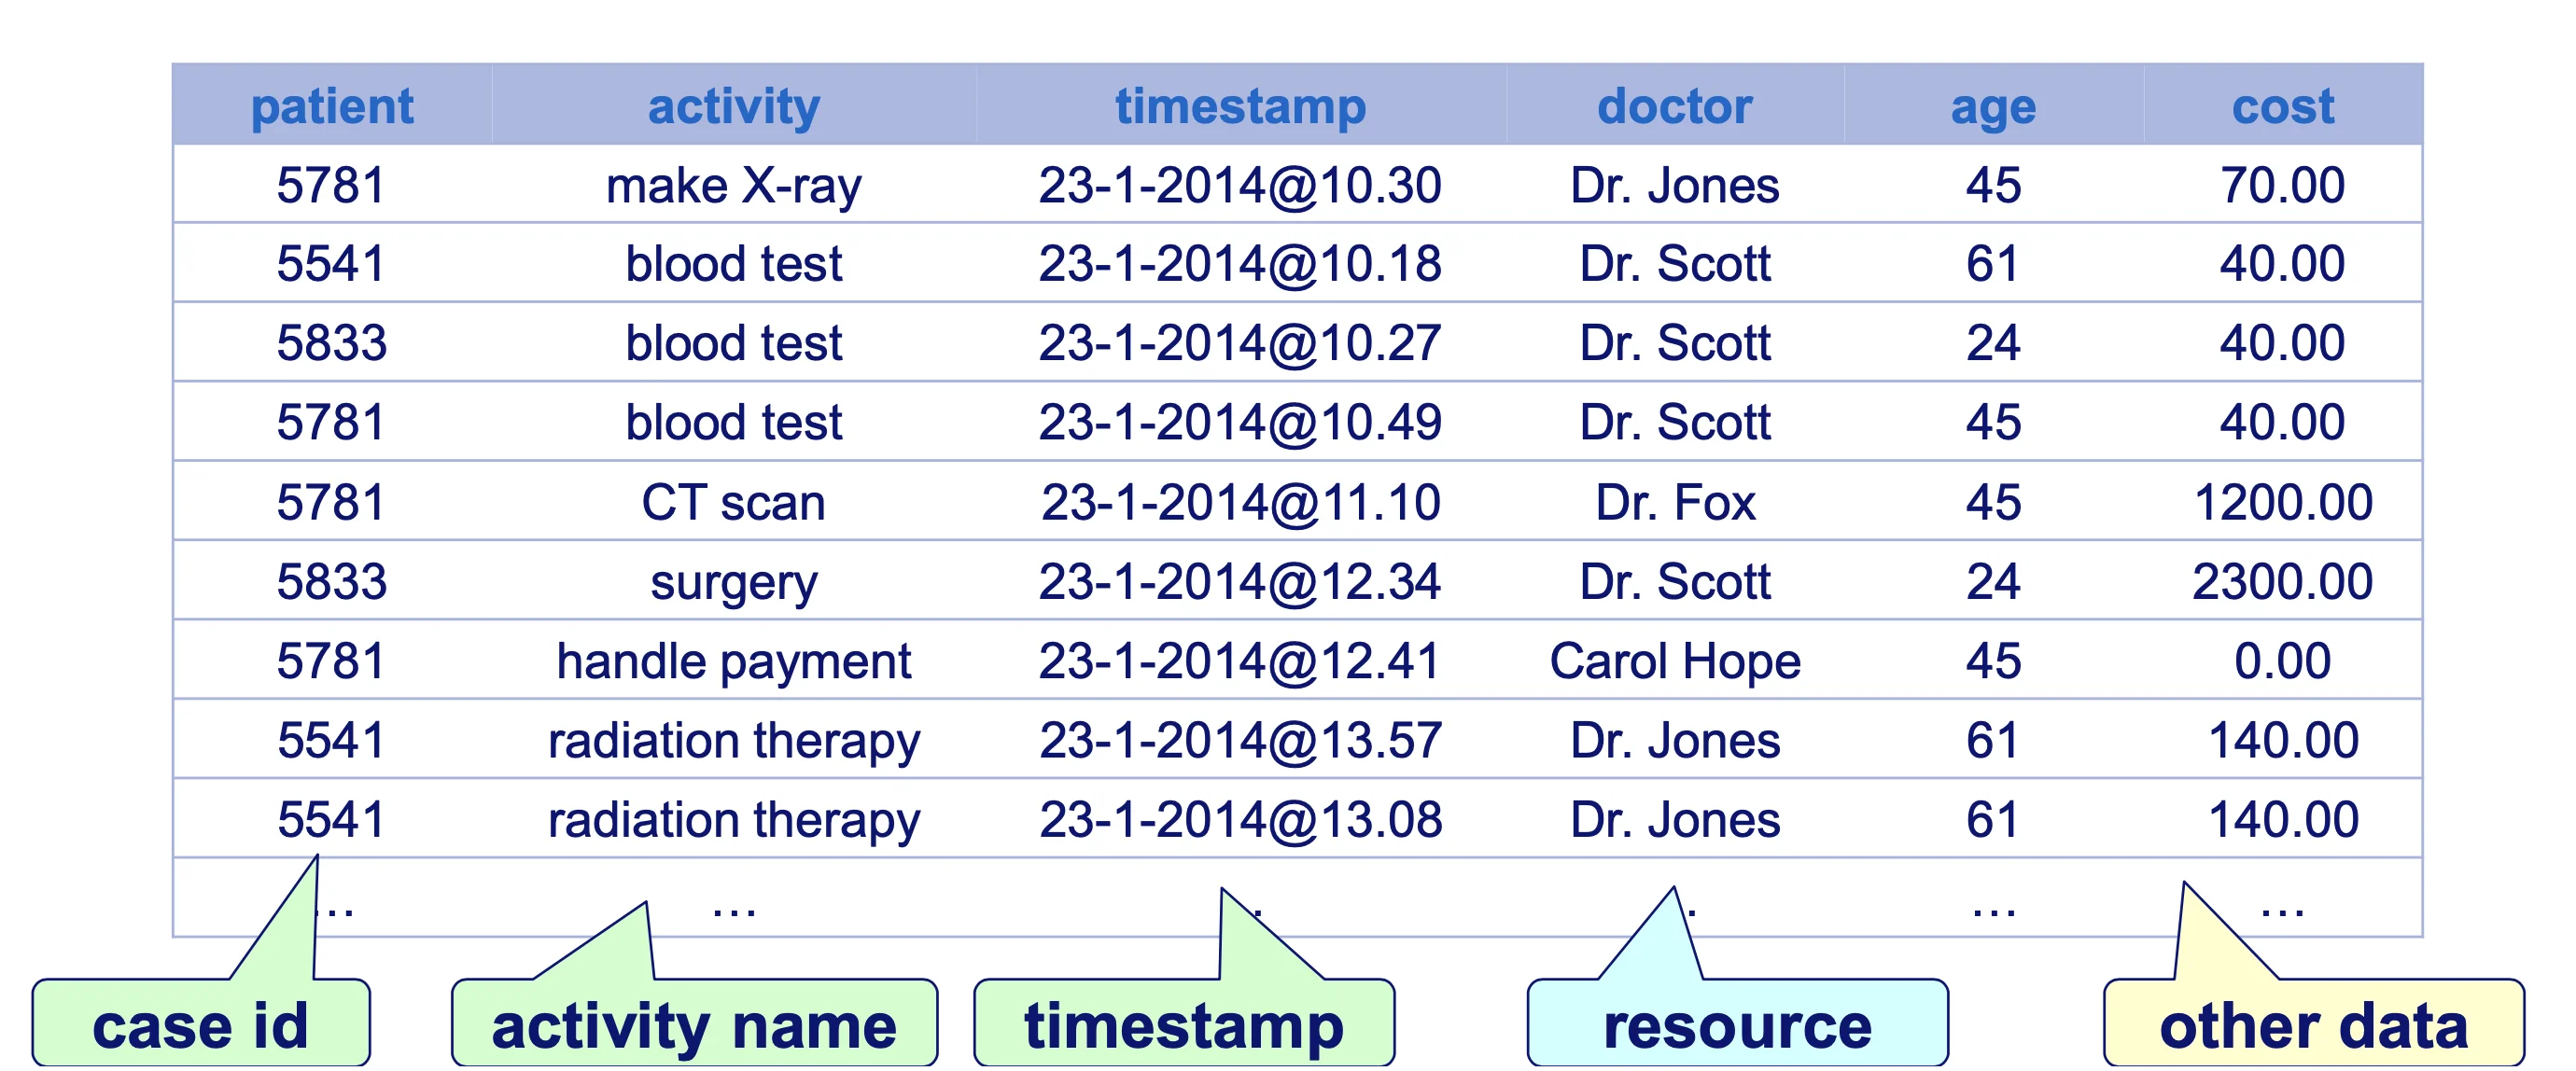
\includegraphics[width=0.9\columnwidth]{immagini/event_log_ex.png} 
    \caption{Esempio di \textit{event log} \cite{site:event-log-img}}
    \label{fig:event-log-img}
\end{figure}

Un evento (osservando la figura \ref{fig:event-log-img}) è rappresentato da una singola "riga" dell'event log, e contiene informazioni relative a:
\begin{itemize}
\item il caso trattato (identificato dal \textit{case id});
\item l'attività eseguita;
\item il riferimento temporale (\textit{timestamp}).
\end{itemize}
Importante notare come, i campi appena elencati, siano essenziali per descrivere un processo e necessari per rendere un event log utilizzabile in attività di process mining.
Ma un evento può contenere anche altre informazioni aggiuntive (es. risorse, costi, ecc.), queste non sono strettamente necessarie per modellare un processo ma sono comunque utili per effettuare analisi su prospettive diverse.

\subsubsection{Tecniche di process mining}
Le tecniche di process mining si occupano principalmente di:
\begin{itemize}
\item \textit{Process discovery}, con lo scopo di generare un \textit{process model}, ovvero una rappresentazione grafica di un processo, permettendone per la visualizzazione, la documentazione e l'estrazione di informazioni;

\item \textit{Conformance checking}, che confronta il process model con un event log per individuare le differenze e deviazioni, può anche essere utilizzato per valutare la qualità del process model generato durante l'attività di discovery, oppure individuare colli di bottiglia;

\item \textit{Enhancement}, ovvero il miglioramento del process model attraverso l'introduzione di nuove informazioni (es. misure relative alle performance).
\end{itemize}

\begin{figure}[H] 
    \centering 
    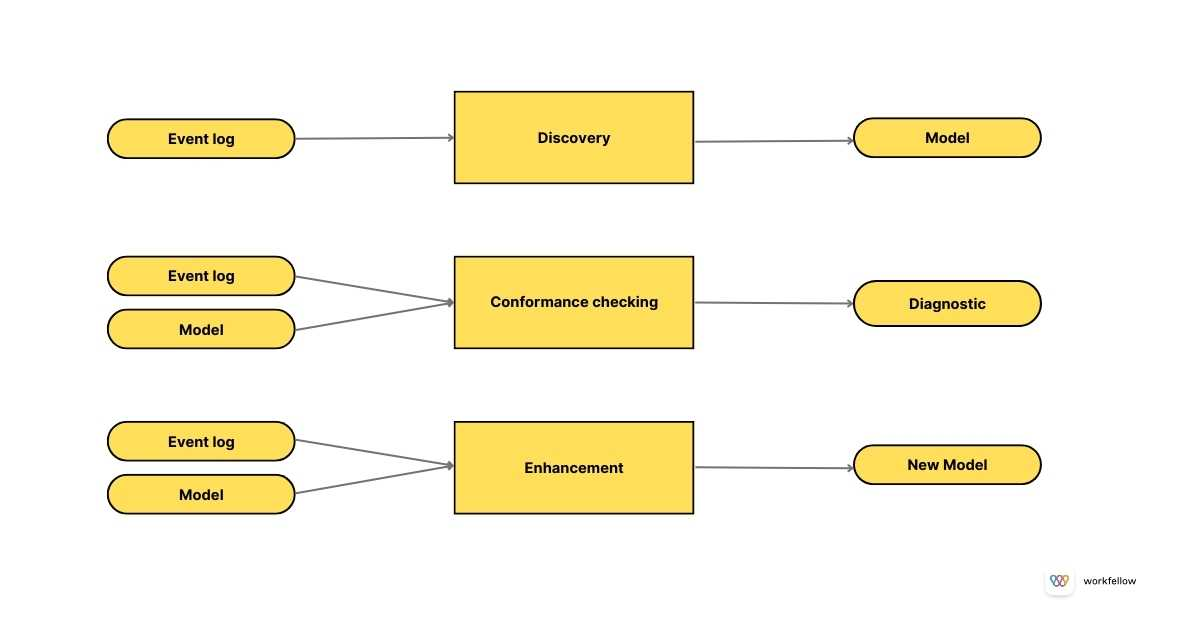
\includegraphics[width=0.9\columnwidth]{immagini/process_mining_techniques.jpg} 
    \caption{3 tipi di attività nel process mining, con relativi input e output \cite{site:process-mining-techniques-img}}
\end{figure}

Le tecniche appena descritte hanno il potenziale di generale un grande valore aggiunto. La creazione di un modello che descrive i processi rende l'individuazione di processi ripetitivi e inefficienti più semplice, permettendo di agire su di essi. Il modello a sua volta può continuamente essere affinato con informazioni aggiuntive che permettono di analizzare le performance e costruire workflow più efficienti. Lo stesso modello può poi essere comparato con event log successivi per individuare deviazioni, mostrando dove, quando e perché accadono. 
\\
Ovviamente, oltre a individuare i problemi e i punti deboli ottimizzabili, il process mining permette anche di scovarli in maniera precoce.
\\
Riassumendo, l'applicazione delle tecniche offerte dal process mining offre vantaggi come: l'ottimizzazione del workflow, la riduzione dei costi, incremento della qualità di beni o servizi offerti e la crescita della soddisfazione del cliente.


\subsection{Predictive Process Monitoring}
Il \textit{Predictive Process Monitoring} rientra tra le attività di Enhancement, ed è una branca del process mining che ha lo scopo di predire il futuro di una esecuzione in corso (e quindi ancora incompleta) di un processo \cite{pm-handbook}.
\\
Generalmente si è interessati a fare predizioni sul tempo totale di esecuzione, sulle attività successive o sui risultato finale del processo.
\\
Questo permette di ottimizzare le operazioni di business, riducendo i costi e i rischi. Inoltre rende la pianificazione in materia di allocazione delle risorse disponibili più semplice ed efficiente.
Importante è anche i benefici relativi alla soddisfazione del cliente: posso fare predizioni relative alle aspettative dei clienti o prevedere il risultato finale di un processo, offrendo tempi di attesa più certi. 
\\
Come osservato in \cite{pm-handbook}, in generale il Predictive Process Monitoring è svolto in due fasi:
\begin{itemize}
\item la fase di \textit{training}: dove viene allenato un modello predittivo (tramite tecniche di Machine Learning) su dati storici di esecuzione, dove le tracce sono complete;
\item la fase di \textit{runtime}: dove il modello predittivo creato viene interrogato con lo scopo di ottenere predizioni relative a tracce incomplete e/o in corso di esecuzione.
\end{itemize}

\subsection{Prescriptive Process Monitoring}
Va osservata la differenze tra predizione, ovvero un'affermazione che spiega ciò che, probabilmente, avverrà (o meno) in futuro e una raccomandazione, ovvero un'affermazione che spiega quale sia la miglior azione da scegliere.
Lo scopo finale del Predictive Process Monitoring è infatti, quello di offrire una predizione relativa all'ottenimento di un risultato positivo, ma non dice niente in relazione a quale sia l'azione successiva migliore da effettuare.
\\
Il Prescriptive Process Monitoring si pone questo obiettivo, supportando e offrendo raccomandazioni agli stakeholder per prevenire risultati indesiderati o per determinare quali sono le migliori attività da eseguire per ottimizzare determinati aspetti di interesse \cite{pm-handbook}.


\subsection{Sistema di raccomandazione per istanze di processi aziendali}
Un sistema di raccomandazione per istanze di processi aziendali, o PAR, è una tipologia di sistema informativo che ha lo scopo di prevedere come le istanze di processi andranno ad evolversi e raccomandare le azioni necessarie per correggere le istanze con il rischio più alto di non raggiungere il risultato desiderato, definito in termini di \gls{KPI} \cite{paper-padella}.
\\
Un sistema PAR (come descritto in \cite{paper-padella}) è composto da due sotto-sistemi: il Predictive Process Monitoring che si occupa di generare le predizioni e il Prescriptive Process Monitoring che genera le raccomandazioni relative alle azioni correttive da applicare.
\\
Sempre in \cite{paper-padella} viene fatta un'importante osservazione: le raccomandazioni, se non correttamente spiegate, spingono l'utente a diffidare di esse, aumentando il rischio che queste non vengano applicate, dato che i responsabili preferiranno prendere decisioni soggettive non fidandosi del sistema.
\\
Quindi la sola raccomandazione non basta, è importante che le ragioni che la determinano siano spiegate e rese comprensibili, così da far sentire l'utente partecipe nelle decisioni prese dal sistema e di conseguenza aumentare la fiducia in esso.
\\
Le spiegazioni del sistema proposto in \cite{paper-padella} si basano su caratteristiche relative al processo come il valore delle sue variabili, le attività effettuate e le risorse sfruttate per svolgere le attività. Il sistema utilizza i valori di Shapley (in inglese \textit{Shapley Values}) per fornire le spiegazioni, concentrandosi solamente sugli aspetti il cui impatto negativo viene maggiormente mitigato della raccomandazione.


\subsubsection{Shapley Values}
Gli Shapley Values nascono nell'ambito della teoria dei giochi, e rappresentano un approccio per suddividere equamente la ricompensa tra i giocatori che hanno collaborato in un gioco cooperativo \cite{site:wiki-shapley-values}. Servono quindi per quantificare la contribuzione che ogni giocatore ha portato al gioco stesso. In \cite{paper-padella} viene spiegato come le caratteristiche di un istanza di processo corrispondano ai giocatori, e la differenza tra la predizione fatta dal modello predittivo e la predizione media è la ricompensa. Quindi il valore di Shapley di una caratteristica di una predizione rappresenta quanto essa contribuisce a variare la predizione del modello da quella media.

\section{Struttura del resto della relazione}
%TODO

